% Sección 6. Contenido: Sara Albarracín (#34, docs/EDA_HALLAZGOS.md); integración en LaTeX: Juan Diego (#39).
% Cifras: outputs/eda/ (resumen_eda.json, temporal_*.csv, territorial_*.csv, atipicos_*.csv,
% fuentes_correlacion_*.csv). Figuras: copias de outputs/eda/figuras/. Se regeneran con scripts/eda.py.

\section{Análisis exploratorio}\label{sec:eda}

El análisis exploratorio lo ejecuta \texttt{scripts/eda.py} sobre los conjuntos de la sección~\ref{sec:preprocesamiento}. Tiene tres bloques:
\begin{itemize}
  \item el \textbf{temporal}, sobre la serie objetivo: 2.131 días, del 2020-01-01 al 2025-10-31, con una media de 343,0 víctimas al día;
  \item el \textbf{territorial}, sobre la Línea 123, la única fuente con resolución dentro de la ciudad;
  \item la \textbf{relación entre las tres fuentes}, en mes $\times$ Bogotá, la única resolución común.
\end{itemize}
Las cifras de esta sección están en \texttt{outputs/eda/}.

\subsection{Evolución anual}\label{sec:eda-anual}

La tabla~\ref{tab:eda-anual} resume cada año de la serie. Sus víctimas, días y medias diarias son las de la tabla~\ref{tab:anual}, con otro redondeo en la media; esa tabla añade los registros del archivo antes del corte (sección~\ref{sec:objetivo}). Aquí se leen para ver cómo cambia el nivel de un año a otro.

\begin{table}[H]
\centering
\caption{Víctimas registradas por año. Fuente: \texttt{outputs/\allowbreak{}eda/\allowbreak{}temporal\_\allowbreak{}anual.csv}.}\label{tab:eda-anual}
\small
\begin{tabular}{@{}lrrrl@{}}
\toprule
\textbf{Año} & \textbf{Víctimas} & \textbf{Media diaria} & \textbf{Días} & \textbf{Año completo} \\
\midrule
2020 & 83.136 & 227,1 & 366 & Sí \\
2021 & 109.428 & 299,8 & 365 & Sí \\
2022 & 137.157 & 375,8 & 365 & Sí \\
2023 & 158.745 & 434,9 & 365 & Sí \\
2024 & 130.503 & 356,6 & 366 & Sí \\
2025 & 111.901 & 368,1 & 304 & No: termina el 31 de octubre \\
\bottomrule
\end{tabular}
\end{table}

\textbf{2020 no es un año típico.} Con 227,1 víctimas diarias queda un 48\,\% por debajo de 2023, el año más alto. Su nivel coincide con las restricciones de movilidad, así que no se lee como el punto de partida de una tendencia. Por eso entra en el modelado con el indicador de año atípico (sección~\ref{sec:variables}).

\textbf{El total de 2025 no es comparable, pero su media diaria sí.} La serie se corta el 2025-10-31, así que 2025 tiene 304 días. Su total sugiere una caída, pero su media diaria, 368,1, supera la de 2024, que fue de 356,6. Mientras el último año esté truncado, el informe compara medias diarias y no totales.

\subsection{Perfil semanal y festivos}\label{sec:eda-semana}

La figura~\ref{fig:eda-semana} muestra la media de víctimas por día de la semana. El viernes es el día más alto, con 403,1, y el domingo el más bajo, con 245,0: un 65\,\% más. Es la señal más fuerte de la serie, y por eso el día de la semana es una predictora.

\begin{figure}[H]
\centering
\IfFileExists{figuras/eda_dia_semana.pdf}{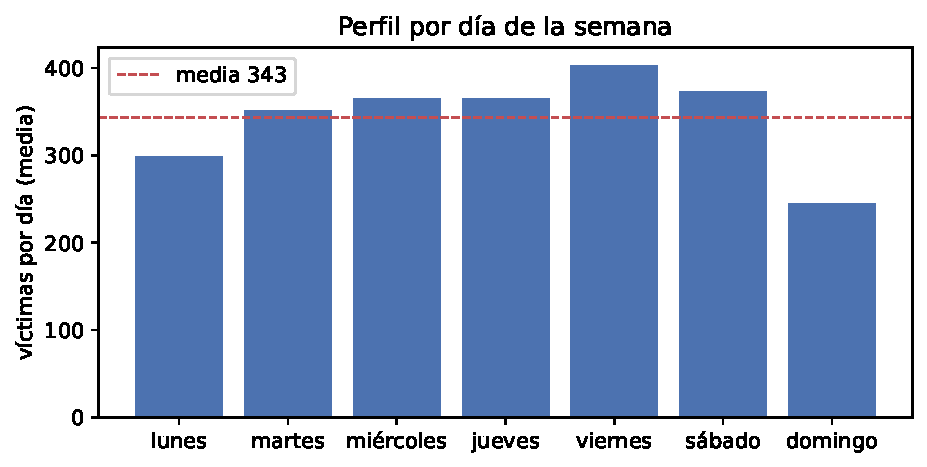
\includegraphics[width=0.72\textwidth]{figuras/eda_dia_semana.pdf}}{\fbox{Figura pendiente: \texttt{figuras/eda\_dia\_semana.pdf}}}
\caption{Media de víctimas registradas por día de la semana, 2020-01-01 a 2025-10-31. La línea discontinua es la media de la serie. Fuente: \texttt{outputs/\allowbreak{}eda/\allowbreak{}temporal\_\allowbreak{}dia\_\allowbreak{}semana.csv}.}\label{fig:eda-semana}
\end{figure}

La fuerza del perfil semanal no implica que repetir el valor de hace siete días sea siempre el mejor comparador trivial. En la validación de origen rodante, el ingenuo de un día gana cuatro de los seis pliegues (sección~\ref{sec:barra}). La regularidad semanal se debilita de noviembre a enero, y por eso la barra se calcula sobre el conjunto en que se evalúa.

\textbf{Los festivos.} En un festivo se registran en promedio 203,6 víctimas, frente a 350,1 en un día no festivo. Esa comparación mezcla dos efectos: la Ley 51 de 1983 traslada muchos festivos al lunes, que ya es un día bajo. Para separarlos, la tabla~\ref{tab:eda-festivos} compara lunes con lunes.

\begin{table}[H]
\centering
\caption{Lunes festivos frente a lunes laborables. Fuente: \texttt{outputs/\allowbreak{}eda/\allowbreak{}resumen\_\allowbreak{}eda.json}.}\label{tab:eda-festivos}
\small
\begin{tabular}{@{}lrr@{}}
\toprule
 & \textbf{Media de víctimas} & \textbf{Lunes} \\
\midrule
Lunes festivo & 201,5 & 62 \\
Lunes laborable & 323,9 & 242 \\
\midrule
Diferencia & $-$37,8\,\% & \\
\bottomrule
\end{tabular}
\end{table}

El efecto se sostiene al controlar el día de la semana: un lunes festivo registra un 38\,\% menos de víctimas que un lunes laborable. El periodo tiene 103 festivos. El calendario de festivos se conoce de antemano, así que usarlo como predictora no introduce información futura.

\subsection{Estacionalidad mensual}\label{sec:eda-mes}

La figura~\ref{fig:eda-mes} muestra la media diaria por mes. Va de 312,7 en abril a 386,9 en octubre, un 24\,\% entre el mínimo y el máximo, frente al 65\,\% del perfil semanal. La estacionalidad mensual existe, pero es mucho más débil que la semanal. Eso sugiere que un modelo con rezagos semanales y calendario captará la mayor parte de la estructura de la serie. Noviembre aparece alto, con 382,1, porque solo promedia los noviembres de 2020 a 2024: el de 2025 está fuera de la serie.

\begin{figure}[H]
\centering
\IfFileExists{figuras/eda_estacionalidad_mensual.pdf}{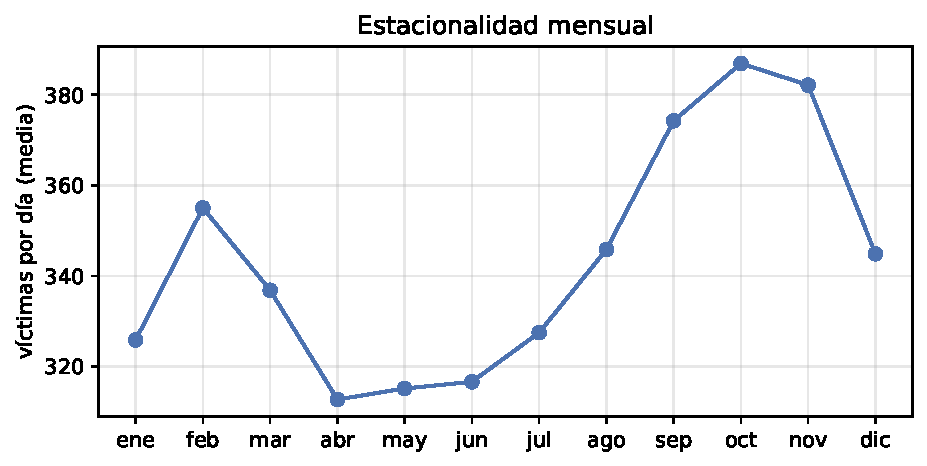
\includegraphics[width=0.72\textwidth]{figuras/eda_estacionalidad_mensual.pdf}}{\fbox{Figura pendiente: \texttt{figuras/eda\_estacionalidad\_mensual.pdf}}}
\caption{Media diaria de víctimas registradas por mes, 2020-01-01 a 2025-10-31. El eje vertical no empieza en cero. Fuente: \texttt{outputs/\allowbreak{}eda/\allowbreak{}temporal\_\allowbreak{}mes.csv}.}\label{fig:eda-mes}
\end{figure}

\subsection{Valores atípicos}\label{sec:eda-atipicos}

Para detectar días atípicos, cada día se compara con la media y la desviación de su propio día de la semana. Un percentil sobre toda la serie no serviría: el perfil semanal domina, y un domingo con 300 víctimas es alto mientras que un viernes con 300 es bajo. Ese percentil, además, marcaría como atípicos los días normales de los años altos.

Con un umbral de $|z| > 3$ hay 10 días atípicos de 2.131, el 0,47\,\%. Ocho de los nueve bajos caen en marzo y abril de 2020, durante el confinamiento estricto; la tabla~\ref{tab:eda-atipicos} muestra los cinco más extremos. El noveno es el 25 de diciembre de 2024, Navidad, con 70 víctimas frente a una media de 365,0 para un miércoles ($z = -3{,}04$). Dos de los nueve son festivos: el Jueves Santo de 2020 (9 de abril) y esa Navidad.

\begin{table}[H]
\centering
\caption{Los cinco días atípicos más bajos, comparados con la media de su día de la semana. Fuente: \texttt{outputs/\allowbreak{}eda/\allowbreak{}atipicos\_\allowbreak{}bajos.csv}.}\label{tab:eda-atipicos}
\small
\begin{tabular}{@{}llrrr@{}}
\toprule
\textbf{Fecha} & \textbf{Día} & \textbf{Víctimas} & \textbf{Media de su día} & \textbf{$z$} \\
\midrule
2020-03-25 & Miércoles & 34 & 365,0 & $-$3,41 \\
2020-04-09 & Jueves & 36 & 364,8 & $-$3,34 \\
2020-03-31 & Martes & 52 & 351,1 & $-$3,24 \\
2020-03-26 & Jueves & 50 & 364,8 & $-$3,20 \\
2020-04-07 & Martes & 57 & 351,1 & $-$3,18 \\
\bottomrule
\end{tabular}
\end{table}

Los días atípicos no se eliminan, porque no son errores de medición. Los de 2020 son el efecto de una restricción real, que recoge el indicador de año atípico, y el de 2024 es un festivo, que recoge el calendario. El único día atípico alto es el 1 de diciembre de 2022, un jueves, con 678 víctimas frente a una media de 364,8 ($z = 3{,}18$). Coincide con el inicio de la temporada de compras de fin de año, pero con un solo día esa explicación no se puede verificar (\texttt{outputs/\allowbreak{}eda/\allowbreak{}atipicos\_\allowbreak{}altos.csv}).

\subsection{Distribución territorial}\label{sec:territorial}

Solo la Línea 123 tiene resolución dentro de la ciudad, así que este bloque describe llamadas tramitadas y no víctimas registradas. Como en la sección~\ref{sec:datos}, el volumen es la suma de \texttt{CANT\_INCIDENTES} y el periodo es 2020--2025. En total son 821.304 incidentes: 815.621 tienen localidad y 5.683, el 0,69\,\%, quedan como «SIN LOCALIZACION». Estos últimos se separan, porque no corresponden a ninguna localidad ni tienen población con la que calcular una tasa.

\subsubsection*{Conteo frente a tasa}

Por conteo, las cinco primeras localidades son Kennedy (99.525 incidentes, 12,12\,\%), Engativá (93.654; 11,40\,\%), Suba (93.132; 11,34\,\%), Bosa (52.210; 6,36\,\%) y Usaquén (50.245; 6,12\,\%) (\texttt{outputs/\allowbreak{}eda/\allowbreak{}territorial\_\allowbreak{}localidad.csv}). Ese orden refleja sobre todo el tamaño de cada localidad.

Para comparar localidades de tamaño distinto se calcula la tasa de llamadas por 100.000 habitantes. La tasa divide los incidentes de 2020--2025 por las personas-año del mismo periodo, con la población de cada año (sección~\ref{sec:poblacion}). Cruzan las 20 localidades. La figura~\ref{fig:eda-tasa} muestra el resultado, y la tabla~\ref{tab:eda-tasa} recoge las localidades que más cambian de puesto.

\begin{figure}[H]
\centering
\IfFileExists{figuras/eda_localidad_tasa.pdf}{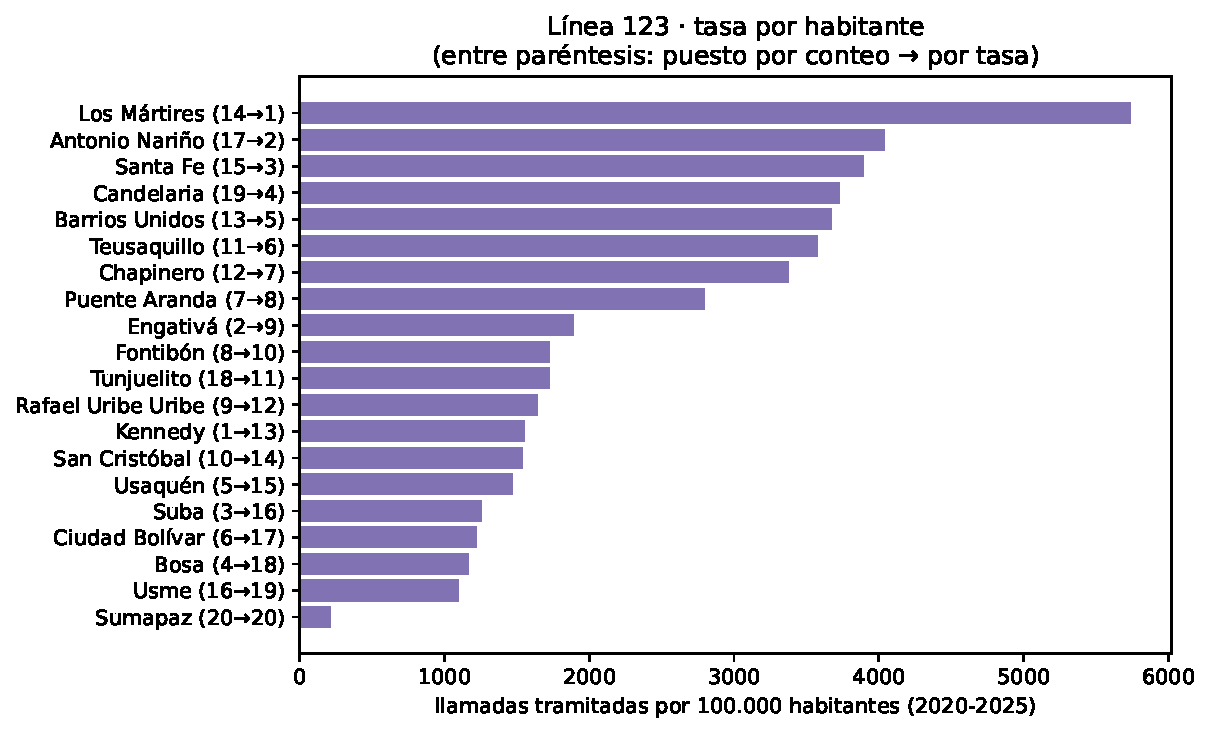
\includegraphics[width=0.85\textwidth]{figuras/eda_localidad_tasa.pdf}}{\fbox{Figura pendiente: \texttt{figuras/eda\_localidad\_tasa.pdf}}}
\caption{Llamadas de hurto tramitadas por la Línea 123 por cada 100.000 habitantes, 2020--2025. Entre paréntesis, el puesto por conteo y el puesto por tasa. Fuente: \texttt{outputs/\allowbreak{}eda/\allowbreak{}territorial\_\allowbreak{}tasas.csv}.}\label{fig:eda-tasa}
\end{figure}

\begin{table}[H]
\centering
\caption{Localidades que más cambian de puesto al pasar del conteo a la tasa. Fuentes: \texttt{outputs/\allowbreak{}eda/\allowbreak{}territorial\_\allowbreak{}tasas.csv} y \texttt{territorial\_\allowbreak{}localidad.csv}.}\label{tab:eda-tasa}
\small
\begin{tabular}{@{}lrrrrr@{}}
\toprule
\textbf{Localidad} & \textbf{Incidentes} & \textbf{Personas-año} & \begin{tabular}[b]{@{}r@{}}\textbf{Tasa por}\\\textbf{100.000}\end{tabular} & \begin{tabular}[b]{@{}r@{}}\textbf{Puesto}\\\textbf{por conteo}\end{tabular} & \begin{tabular}[b]{@{}r@{}}\textbf{Puesto}\\\textbf{por tasa}\end{tabular} \\
\midrule
Los Mártires & 29.033 & 506.159 & 5.735,9 & 14 & 1 \\
Antonio Nariño & 19.521 & 483.662 & 4.036,1 & 17 & 2 \\
Santa Fe & 25.991 & 667.201 & 3.895,5 & 15 & 3 \\
La Candelaria & 3.834 & 102.815 & 3.729,0 & 19 & 4 \\
\midrule
Engativá & 93.654 & 4.953.028 & 1.890,8 & 2 & 9 \\
Kennedy & 99.525 & 6.412.231 & 1.552,1 & 1 & 13 \\
Suba & 93.132 & 7.420.285 & 1.255,1 & 3 & 16 \\
Bosa & 52.210 & 4.485.744 & 1.163,9 & 4 & 18 \\
\bottomrule
\end{tabular}
\end{table}

\textbf{El orden cambia por completo.} Kennedy pasa del primer puesto por conteo al decimotercero por tasa. Los Mártires, decimocuarta por conteo, es la primera por tasa, con 3,7 veces la tasa de Kennedy. La Candelaria es el caso extremo: con 3.834 incidentes es la penúltima por conteo y la cuarta por tasa. Es la localidad con menos habitantes después de Sumapaz, y el conteo la ocultaba. El conteo mide sobre todo el tamaño de la población, no la intensidad del fenómeno.

La figura~\ref{fig:eda-mapa} representa la tasa en el mapa, y no el conteo. Un mapa de conteos destacaría las localidades más pobladas y sugeriría que son las más peligrosas. Con la tasa, el centro de la ciudad aparece como la zona con más llamadas por habitante, y las localidades grandes del sur y el occidente quedan en valores intermedios.

\begin{figure}[H]
\centering
\IfFileExists{figuras/eda_mapa_tasa.pdf}{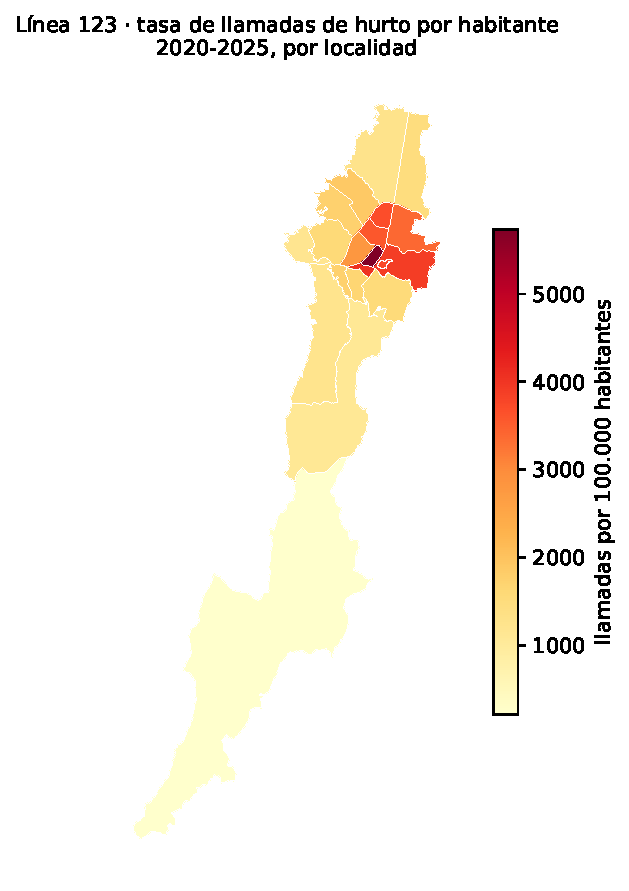
\includegraphics[width=0.5\textwidth]{figuras/eda_mapa_tasa.pdf}}{\fbox{Figura pendiente: \texttt{figuras/eda\_mapa\_tasa.pdf}}}
\caption{Tasa de llamadas de hurto a la Línea 123 por 100.000 habitantes y por localidad, 2020--2025. Geometrías: Secretaría Distrital de Seguridad, Convivencia y Justicia (\texttt{data/README.md}). Fuente: \texttt{outputs/\allowbreak{}eda/\allowbreak{}territorial\_\allowbreak{}tasas.csv}.}\label{fig:eda-mapa}
\end{figure}

\subsubsection*{Lo que la tasa no mide}

\begin{enumerate}
  \item \textbf{No es una tasa de hurtos.} La Línea 123 cuenta llamadas tramitadas, así que la tasa mide la demanda de atención por habitante y no la victimización.
  \item \textbf{No incluye la población flotante.} Los Mártires, Santa Fe, La Candelaria, Chapinero y Teusaquillo reciben cada día a muchas personas que no viven en ellas, por trabajo, comercio o transporte, y ocupan los puestos 1, 3, 4, 6 y 7 por tasa. A Antonio Nariño, en el 2.º, le aplica lo mismo, porque también concentra comercio y transporte. Como el denominador es la población residente, su tasa se sobrestima. Sin una medida de población flotante no se puede separar ese efecto, así que el orden por tasa no se interpreta como el riesgo de quienes están en la localidad.
  \item \textbf{La tasa de Sumapaz es inestable.} Es una localidad rural, con la menor población de la ciudad y 38 incidentes en todo el periodo. Con tan pocos casos, su tasa de 213,3 por 100.000 cambia mucho por un solo incidente.
  \item \textbf{Ninguno de los dos órdenes mide peligrosidad.} El conteo y la tasa describen dónde se pide atención, cada uno con su propio sesgo. Se presentan los dos para mostrar cuánto cambia el orden al normalizar.
\end{enumerate}

\subsubsection*{Unidades de planeamiento zonal}

La UPZ es la resolución más fina del proyecto, y solo la Línea 123 la tiene. En 2020--2025, 723.282 incidentes tienen una UPZ asignada, repartidos en 116 UPZ; el resto de los incidentes con localidad figura como «SIN UPZ» y se separa (\texttt{outputs/\allowbreak{}eda/\allowbreak{}territorial\_\allowbreak{}upz.csv}). La más frecuente es El Rincón, en Suba, con el 2,80\,\% de esos incidentes. Le siguen La Sabana, en Los Mártires (2,66\,\%), Las Ferias, en Engativá (2,38\,\%), Tibabuyes, en Suba (2,26\,\%), y Bosa Central (2,24\,\%).

Las diez primeras UPZ suman solo el 22,3\,\%. El hurto que se reporta a la Línea 123 está repartido por la ciudad y no concentrado en unos pocos puntos. Para el modelado, eso respalda usar la serie de toda la ciudad, porque ninguna UPZ arrastra el total. Para la interpretación, desaconseja presentar las primeras UPZ como «las más peligrosas»: la diferencia entre la primera y la décima es pequeña.

\subsection{Relación entre las tres fuentes}\label{sec:fuentes-eda}

Las tres fuentes se comparan en mes $\times$ Bogotá, la única resolución común, durante 70 meses, de 2020-01 a 2025-10. No se suman: se comparan sus series, cada una en su unidad. La figura~\ref{fig:eda-fuentes} las normaliza dividiendo cada una por su media, y la tabla~\ref{tab:eda-corr} da sus correlaciones.

\begin{figure}[H]
\centering
\IfFileExists{figuras/eda_fuentes_normalizadas.pdf}{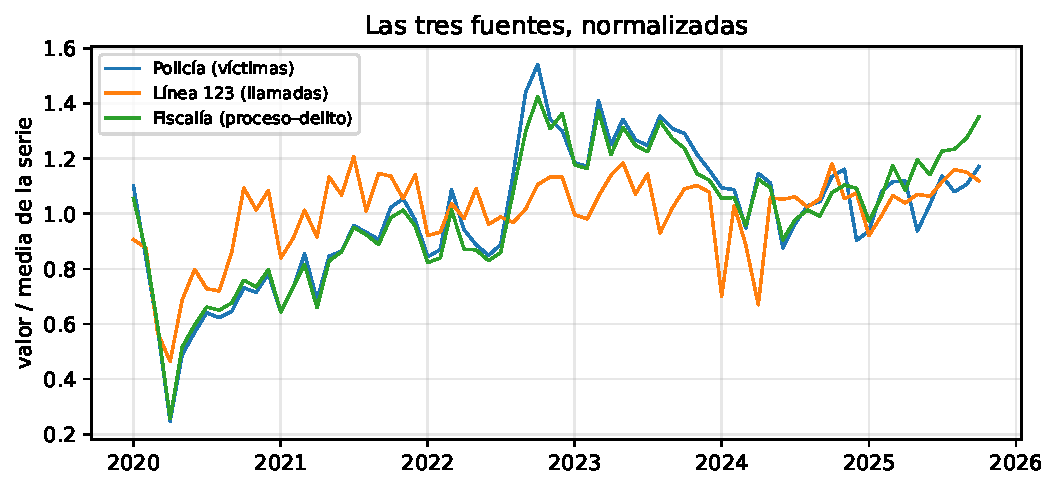
\includegraphics[width=\textwidth]{figuras/eda_fuentes_normalizadas.pdf}}{\fbox{Figura pendiente: \texttt{figuras/eda\_fuentes\_normalizadas.pdf}}}
\caption{Series mensuales de las tres fuentes, divididas por su media, 2020-01 a 2025-10. Policía: víctimas; Línea 123: llamadas; Fiscalía: filas proceso--delito. Fuente: \texttt{outputs/\allowbreak{}informe/\allowbreak{}series\_\allowbreak{}mensuales\_\allowbreak{}fuentes.csv}.}\label{fig:eda-fuentes}
\end{figure}

\begin{table}[H]
\centering
\caption{Correlación entre las series mensuales: 2020-01 a 2025-10 (70 meses) y la misma ventana sin 2020 (58 meses). Fuente: \texttt{outputs/\allowbreak{}eda/\allowbreak{}fuentes\_\allowbreak{}correlacion\_\allowbreak{}pearson.csv}, \texttt{fuentes\_\allowbreak{}correlacion\_\allowbreak{}spearman.csv} y \texttt{fuentes\_\allowbreak{}correlacion\_\allowbreak{}pearson\_\allowbreak{}sin\_\allowbreak{}2020.csv}.}\label{tab:eda-corr}
\small
\begin{tabular}{@{}lrrr@{}}
\toprule
\textbf{Par de fuentes} & \textbf{Pearson} & \textbf{Spearman} & \textbf{Pearson sin 2020} \\
\midrule
Policía -- Fiscalía & 0,962 & 0,947 & 0,925 \\
Fiscalía -- Línea 123 & 0,633 & 0,537 & 0,355 \\
Policía -- Línea 123 & 0,601 & 0,470 & 0,284 \\
\bottomrule
\end{tabular}
\end{table}

Las dos fuentes de registro, Policía y Fiscalía, se mueven casi igual (0,962), mientras que la Línea 123 solo correlaciona moderadamente con ellas (0,601 y 0,633).

Sin 2020, la correlación entre los dos registros apenas cambia (0,925), pero la de la Línea 123 cae a 0,284 con Policía y a 0,355 con Fiscalía. Eso es compatible con que buena parte de su correlación aparente venga de la caída simultánea de las tres fuentes durante el confinamiento: un choque común produce correlación aunque no haya una relación estable entre las series. Fuera de 2020, la Línea 123 es la fuente menos redundante de las tres.

La diferencia entre fuentes es compatible con el origen de cada una. Policía y Fiscalía registran hechos denunciados dentro de sistemas institucionales. La Línea 123 recoge llamadas ciudadanas, que dependen de la decisión de llamar y no de que el caso entre en un sistema. La correlación no prueba ese mecanismo, pero sí respalda dos decisiones ya tomadas:
\begin{itemize}
  \item usar la Línea 123 como contraste para la caída de noviembre y diciembre de 2025, porque es la única fuente que no comparte el mecanismo de registro (sección~\ref{sec:preprocesamiento});
  \item tratar las fuentes como complementarias y no como intercambiables.
\end{itemize}

\subsection{Implicaciones para el modelado}\label{sec:eda-implicaciones}

\begin{enumerate}
  \item \textbf{El día de la semana es la señal dominante}: el viernes registra un 65\,\% más de víctimas que el domingo.
  \item \textbf{Un festivo reduce las víctimas registradas un 38\,\%}, incluso comparando lunes con lunes, y se conoce de antemano.
  \item \textbf{La estacionalidad mensual es débil} frente a la semanal.
  \item \textbf{2020 entra marcado} con el indicador de año atípico. Sus días atípicos son el efecto del confinamiento y no se eliminan. El único atípico bajo fuera de 2020 es la Navidad de 2024, un festivo.
  \item \textbf{Se comparan medias diarias y no totales}, mientras 2025 esté truncado.
  \item \textbf{Las localidades se comparan por tasa y no por conteo}, sin presentar ninguno de los dos órdenes como un ranking de peligrosidad.
  \item \textbf{El fenómeno está disperso en el territorio}, lo que respalda modelar la serie de toda la ciudad.
\end{enumerate}
